\begin{table}[H]
\centering
\caption{Testing set}
\label{tab:words}
\begin{tabular}{lllll}
\hline
on    & off  & stop & clear & load   \\
go & pause & resume & edit  & quit  \\  
\hline  
\end{tabular}
\end{table}

\subsection{Effective recording length}
\label{subsec:rec_length}
%
\begin{figure}
	\centering
	\includegraphics[width=\linewidth]{"figures/linear_multi"}
	\caption{Recognition accuracy versus the recording length (in frames), while using multiple recordings per word for testing. Used feature matching method: linear.}
	\label{fig:multi}
\end{figure}
%
Since our target hardware has extremely limited resources, the first experiment targets the minimum effective recoding length without significant accuracy loss. 

For this experiment a single microcontroller running on continuous power is used. Each word from Table~\ref{tab:words} was recorded on a PC 20 times. The features---normalized FFT-based values---of the first recording are saved in the microcontroller's persistent memory as a signature to perform the feature matching, during the testing. the rest of the recording are used for conducting the experiment.   

Figure~\ref{fig:multi} shows words recognition accuracy when the 19 recordings of each word are played back from the PC speaker. We can concluded that recording beyond \textit{nine frames} do not increase the recognition accuracy; therefore, nine frames recording length is chosen for the rest of the experiments. 

\subsection{Comparison of feature matching methods}
%
\begin{figure}
\centering
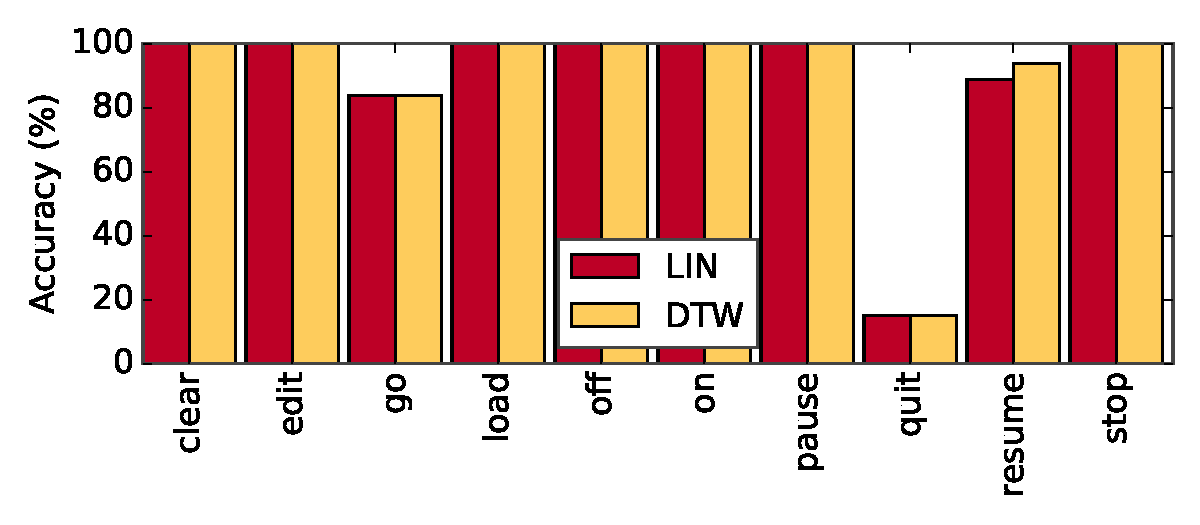
\includegraphics[width=\linewidth]{figures/DTWvsLDM}
\caption{Recognition accuracy for linear matching and DTW when using 9 frames as the recording length.}
\label{fig:DTWvsLDM}
\end{figure}
%
\begin{table}
	\centering
	\caption{Profiling of features matching algorithms: Dynamic Time Warping (DTW) and Linear Distance Matching (LDM)}
	\label{tab:profiling}
	$
	\begin{tabular}{lll}\hline
	Section & Linear (ms) & DTW (ms) \\\hline
	Recording & 285.9  & 285.9 \\
	Feature extraction & 501.9 & 501.9 \\
	Feature matching &  99.4 & 1251 \\\hline
	Total & 887.2 & \\\hline
	\end{tabular}
	$
\end{table}
%
We implemented two algorithms for voice features matching, Dynamic Time Warping (DTW) and Linear Distance Matching (LDM). Due to the microphone wake-on-sound feature and the fixed recording length, DTW did not outperform LDM as Figure~\ref{fig:DTWvsLDM} shows. Moreover, DTW takes more time to process that data as Table~\ref{tab:profiling} shows. Therefore, LDM algorithm is used in future experiments.

\subsection{ Intermittent microphone availability}
%

\begin{figure}
\centering
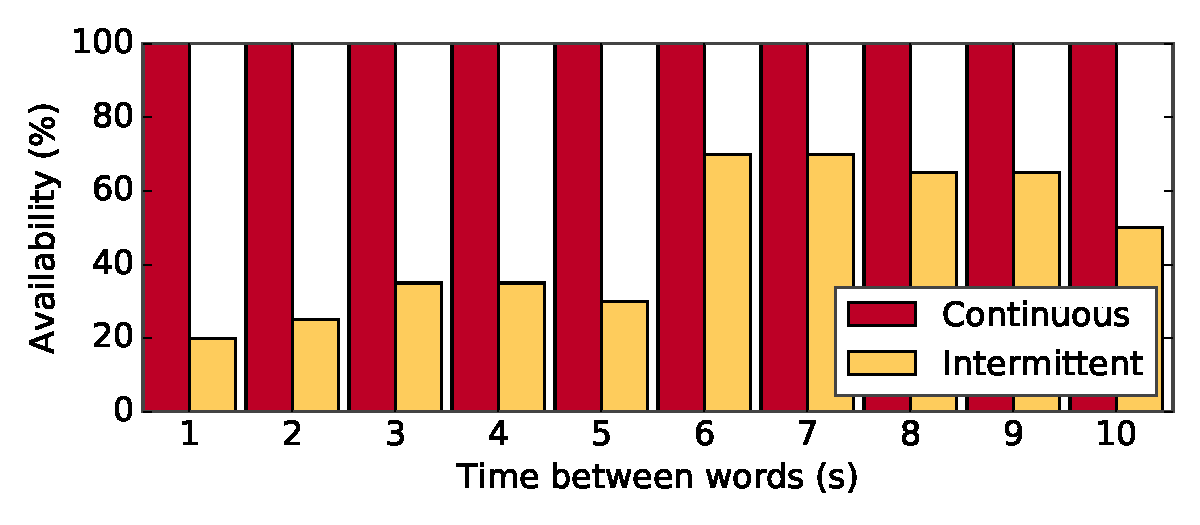
\includegraphics[width=\linewidth]{figures/word_freq}
\caption{The effect of the time between consecutive words on the availability: the percentage of words that is processed by the command recognizer. \todo{Add correct recognition as stacked bar?}}
\label{fig:word_freq}
\end{figure}
%
\begin{table}
	\centering
	\caption{The mean and standard deviation of the parameters that were used to simulate intermittent execution. Here $t_{on}$ is the time the device is on while recording or processing, $t_{off}$ is the time the device is charging and $t_{sleep}$ is the time the device is sleeping while waiting on sound input.}
	\label{tab:simparams}
$
\begin{array}{lll}\hline
\text{Parameter} & \mu \text{ (ms)} & \sigma \text{ (ms)} \\\hline
%t_{rec} & 295 & 0 \\
t_{on} &  590 & 17.7 \\
t_{off} & 5310 & 154 \\
t_{sleep} &  22420 & 652 \\\hline
\end{array}
$
\end{table}
%
This experiment shows the effect of intermittent power supply on a microphone availability \todo{and recognition accuracy} for different command (or word) repetition speed. Each word (from Table~\ref{tab:words}) was played back 20 times with intra-words-playing time ranges from 1 to 10 seconds. 

For the experiment we chose to simulate the intermittent power supply, based on a real measurement, to ensure environment consistency across different words.
In particular, we measured the $t_{on}$; used an on/off ratio of $10\%$ to simulate harsh harvesting conditions~\cite{mementos, harvOS,lucia}; and calculated the $t_{sleep}$ based on the micro controller specification~\cite{datasheet} (Table~\ref{tab:simparams}).     

The obvious observation from Figure~\ref{fig:word_freq} is that intermittency has a great impact on the command recognizer availability. However, a less obvious, but important, observation is that the correlation between the on/off cycle and the command repetition speed has also great impact as the bars labeled with 5 and 6 from Figure~\ref{fig:word_freq} indicate. 





